\documentclass[12pt]{article}
\usepackage[print,nopanel]{pdfscreen}
\begin{print}
\usepackage{lastpage}
\usepackage{macro/macro}

\usepackage{fancyhdr}
\usepackage{verbatim}
\lhead{\large\bfseries eCAD}
\usepackage[left=2.5cm, right=1.5cm, top=1.5cm, bottom=1.5cm]{geometry}
\pagestyle{fancy}
\end{print}
\margins{.5cm}{.5cm}{.5cm}{.5cm}
\begin{screen}
\renewcommand{\encodingdefault}{T1}
\usepackage{setspace}
\linespread{1.5}
\renewcommand{\rmdefault}{ptm}
\end{screen}
\screensize{8cm}{9cm}
\overlay{overlay8.pdf}
\usepackage{graphicx}

\begin{document}
\begin{screen}
\ppttitle
\end{screen}
\footskip 0.7cm
\newpage


\newpage
\section{Introduction}
\subsection{What is eCAD?}
\begin{figure}[h!]
\centering

\includegraphics[width=0.7\textwidth]{images/logo.png}
\caption{eCAD logo}
\end{figure}
eCAD is a fully comprehensive 2D CAD application that you can download and install for free. It is available for major operating systems which includes Microsoft Windows and Linux. It is available in more than 20 languages and for major operating systems which includes Microsoft Windows and Linux.\\\\
The app is great for industrial designers, but anyone who wants to learn how to make 2D
CAD drawings will like this program. For a free software, eCAD gives you a lot of tools
to work with. New users will be able to create basic drawings, while advanced users can
make engineering plans with the software.You can start drawings from scratch. But it is
also easy to put in ellipses, arcs, lines and circles. eCAD also has a powerful zoom tool
that lets you look at models at different distances. This is essential for designers who
are going to make life size copies of a drawing. eCAD also has grids which are extremely
useful for those new to CAD. Once you have made the basic object, you can customize
it in many ways. Scaling is particularly easy here. Also Dimensioning which is must in
every CAD software is there. We can calculate the distance between two points and can
get the size of the object. Here, its worth mentioning about snapping part. We can have
snapping to grid, center etc. One if wants to work by writing a code can do so in scripting
feature. You can download and install eCAD freely, with no fear of copyright infringement.\\\\

\subsection{License}
\begin{figure}[h!]
\centering

\includegraphics[width=0.7\textwidth]{images/gpl.jpg}
\caption{GPLv3}
\end{figure}
The GNU General Public License is a free, copy left license for software and other kinds
of works. The licenses for most software and other practical works are designed to take
away your freedom to share and change the works. The GNU General Public License is a free, copy left license for software and other kinds
of works. The licenses for most software and other practical works are designed to take
away your freedom to share and change the works.\\\\
Then we speak of free software, we are referring to freedom, not price. Our General
Public Licenses are designed to make sure that you have the freedom to distribute copies
of free software (and charge for them if you wish), that you receive source code or can get
it if you want it, that you can change the software or use pieces of it in new free programs,
and that you know you can do these things. For example, if you distribute copies of such a program, whether gratis or for a fee,
you must pass on to the recipients the same freedoms that you received. You must make
sure that they, too, receive or can get the source code. And you must show them these
terms so they know their rights. Developers that use the GNU GPL protect your rights
with two steps:
\begin{itemize}
\item assert copyright on the software
\item offer you this License giving you legal permission to copy, distribute and/or modify
it.
\end{itemize}
For the developer’s and author’s protection, the GPL clearly explains that there is no
warranty for this free software. For both user’s and author’s sake, the GPL requires that
modified versions be marked as changed, so that their problems will not be attributed
erroneously to authors of previous versions.\\\\
For the developer’s and author’s protection, the GPL clearly explains that there is no
warranty for this free software. For both user’s and author’s sake, the GPL requires that
modified versions be marked as changed, so that their problems will not be attributed
erroneously to authors of previous versions.\\\\
Finally, every program is threatened constantly by software patents. States should not
allow patents to restrict development and use of software on general-purpose computers,
but in those that do, we wish to avoid the special danger that patents applied to a free
program could make it effectively proprietary. To prevent this, the GPL assures that
patents cannot be used to render the program non-free.\\\\




 


\newpage
\section{Installation}
To access eCAD we need to follow few steps. There are some prerequisites
needed to run eCAD. The instructions for both Windows and Linux are mentioned below.
\subsection{For Linux}
\begin{enumerate}
\item Downloading
\begin{itemize}
\item Install Qt libraries using sudo apt-get install qtdeclarative5-dev qt5-default
\item Download zip folder of eCAD or clone it from https://github.com/GreatDevelopers/eCAD
\end{itemize}
\item Installing
\begin{itemize}
\item cd eCAD
\item qmake
\item make
\item ./eCAD
\end{itemize}
\end{enumerate}

\subsection{For Windows}
\begin{enumerate}
\item \textbf{Downloading}: Download zip folder of eCAD from https://github.com/GreatDevelopers/eCAD
\item \textbf{Installing}:  Install Qt’s latest version available with mingw compiler from Qt’s official down-
loads. After installation launch Qt creator load eCAD.pro, from the build menu select
‘Build All” and Run.
\end{enumerate}


\newpage
\section{Interface}
\subsection{Menubar}
In eCAD we have menubar. Menubar consists of different menu items and sub menu-items. Each menuitem has its own specific requirements and advantage. Each menu item is described as below:
\begin{figure}[h!]
\centering
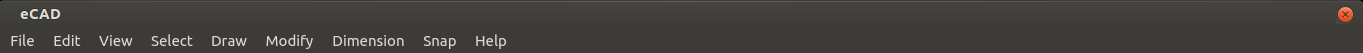
\includegraphics[width=0.9\textwidth]{images/menubar.png}
\caption{Menubar}
\end{figure}
\begin{enumerate}
\item \textbf{File Menu}: It consists of the following submenus.
\begin{itemize}
\item New: On clicking New menuitem we can create a new drawing. The shortcut key to it is Ctrl+N.
\item Open: This option will allow you to open a file which is already saved, so that one can edit it as per user requirement. The shortcut key is Ctrl+O.
\item Save: On clicking this one can save the new file if already not saved or save the existing modified file in xml format. The shortcut to it is Ctrl+S.
\item Save As: The Save As functionality allows to save the new file. The shortcut to it is Ctrl+Shift+S.
\item Import: Using this one can import the file from outside source. One can import jpg and png images in eCAD.
\item Export: Also sometimes the file needs to be exported in different formats. In eCAD one can export the file in the pdf, jpg and png formats.
\item Close: On clicking this the current drawing gets closed.
\item Print preview: Before printing user may want to view the file to print. This can be done by clicking this option or by pressing Ctrl+Shift+P. 
\item Print: To print the file click on it or press Ctrl+P.
\item Quit: To quit or close the software click on it or press Ctrl+Q.
\end{itemize}
\item \textbf{Edit Menu}: It contains the following submenus
\begin{itemize}
\item Cut: To cut the item click on it or press Ctrl+X.
\item Copy: To copy the item click on it or press Ctrl+C.
\item Paste: To paste the item click on it or press Ctrl+V.
\item Undo: To Undo click on it or press Ctrl+Z.
\item Redo: To Redo click on it or press Ctrl+Shift+Z.
\end{itemize}
\item \textbf{View menu}: It contains the following submenus
\begin{itemize}
\item Grid: On checking/unchecking it appears or disappears.
\item Zoom In: This option allows the view to zoom in.
\item Zoom out: On clicking it the view gets zoomed out.
\item Panning: One can scroll the drawing workspace using this feature.
\item Status Bar: This shows the current mouse position and also specifies the instructions to draw the entities.
\item Tool Bar: It futher have submenus for toolbar, scripting widgets and console mode.
\end{itemize}
\item \textbf{Select}: It contains the following submenus
\begin{itemize}
\item Select all: This will select all the entities
\item Deselect all: This will deselect all entites 
\item Select Window: This will select full window
\item Select entity: This will allow to select one entity
\item Deselect window: This will deselect window 
\item Invert Selection: This will invert the selection.
\end{itemize}
\item \textbf{Draw}: It contains the following submenus
\begin{itemize}
\item Points: It is used to draw points.
\item Line: It is used to draw Line.
\item Circle: It is used to draw Circle.
\item Ellipse: It is used to draw ellipse.
\item Arc: It is used to draw arc.
\item Text: It is used to add the text.
\item Image: It is used to add the image.
\end{itemize}
\item \textbf{Modify} : It contains the following submenus
\begin{itemize}
\item Delete selected: It will delete all the selected items.
\item Delete entity: It will delete the single entity. 
\end{itemize}
\item \textbf{Dimension}: It contains the following submenus
\begin{itemize}
\item Horizontal: It will allow to do the horizontal dimensioning.
\item Vertical: It allows to do vertical dimensioning.
\item Radial: It allows radial dimensioning too.
\item Diametric: It has an option for diametric dimensioning too.
\end{itemize}
\item \textbf{Snap}: It contains the following submenus
\begin{itemize}
\item Free: It will be free snap.
\item Grid: It will be for snap to grid. 
\item Center: It will be for snap to center
\item Middle Points: It will be for snap to mid points
\item End points: It will be for snap to end points
\end{itemize}
\item \textbf{Help}: It contains following submenus
\begin{itemize}
\item Manual: It will open the manual of the eCAD, that you are currently reading.
\item About: It will give brief description regarding license and developers of eCAD.
\end{itemize}
\end{enumerate}
\newpage
\subsection{Toolbar}
\begin{figure}[h!]
\centering

\includegraphics[width=0.9\textwidth]{images/toolbar.png}
\caption{Toolbar}
\end{figure}
Toolbar contains the shortcuts to various items in menubar. Like new, open, save, close, undo, redo etc. There are two toolbar standard toolbar and main toolbar.
\begin{enumerate}
\item \textbf{Main Toolbar}
\begin{figure}[h!]

\includegraphics[width=0.05\textwidth]{images/newDrawing.jpg} 
This creates a new drawing.
\end{figure}
\begin{figure}[h!]

\includegraphics[width=0.05\textwidth]{images/openDrawing.jpg} 
This opens a drawing.
\end{figure}
\begin{figure}[h!]

\includegraphics[width=0.05\textwidth]{images/saveDrawing.jpg} 
This saves a drawing.
\end{figure}
\begin{figure}[h!]

\includegraphics[width=0.05\textwidth]{images/cut.jpg} 
This cuts the selected entity.
\end{figure}
\begin{figure}[h!]

\includegraphics[width=0.05\textwidth]{images/copy.jpg} 
This copies the selected entity.
\end{figure}
\begin{figure}[h!]

\includegraphics[width=0.05\textwidth]{images/paste.jpg} 
This paste the entity at the position.
\end{figure}
\begin{figure}[h!]

\includegraphics[width=0.05\textwidth]{images/undo.jpg} 
This undo the previous action.
\end{figure}
\begin{figure}[h!]

\includegraphics[width=0.05\textwidth]{images/redo.jpg} 
This redo the previous action.
\end{figure}
\item \textbf{Standard ToolBar}
\begin{figure}[h!]

\includegraphics[width=0.05\textwidth]{images/point.jpg} 
This will create points
\end{figure}
\begin{figure}[h!]

\includegraphics[width=0.05\textwidth]{images/line.jpg} 
This will create line
\end{figure}
\begin{figure}[h!]

\includegraphics[width=0.05\textwidth]{images/circle.jpg} 
This will create circle
\end{figure}
\begin{figure}[h!]

\includegraphics[width=0.05\textwidth]{images/ellipse.jpg} 
This will create ellipse
\end{figure}
\begin{figure}[h!]

\includegraphics[width=0.05\textwidth]{images/arc.jpg} 
This will create arc
\end{figure}
\begin{figure}[h!]

\includegraphics[width=0.05\textwidth]{images/text.jpg} 
This will insert text using text editor interaction.
\end{figure}
\begin{figure}[h!]

\includegraphics[width=0.05\textwidth]{images/image.jpg} 
This will insert an image.
\end{figure}
\end{enumerate}
\vspace{30em}
\subsection{Working Space}
\begin{figure}[h!]
\centering
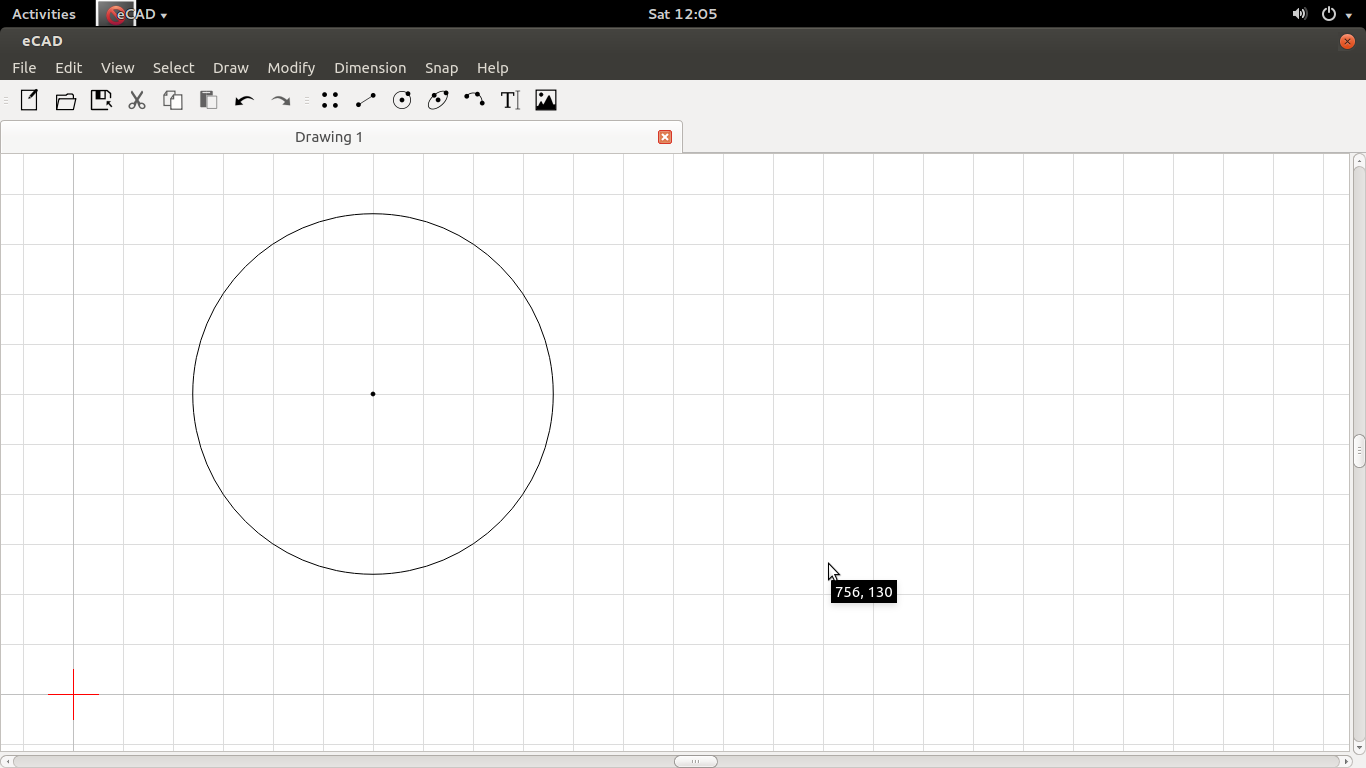
\includegraphics[width=0.9\textwidth]{images/drawingarea.png} 
\caption{Working Space}
\end{figure}
This is the working space where all the entities are drawn. One can increase or decrease the working area by closing or opening the widgets like scripting console and status bar. At present they are closed. This is the maximum area one will get to work. One can also make more than one drawing so that he/she can work easily. All depends upon user needs.
\subsection{Scripting Console}
\begin{figure}[h!]
\centering
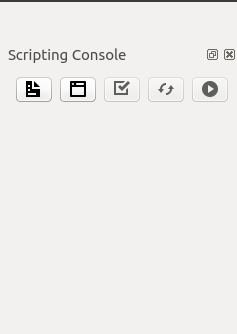
\includegraphics[width=0.4\textwidth]{images/scriptingconsole.png} 
\caption{Scripting console}
\end{figure}
In scripting console user can write the script/code to draw the drawing. So this feature is effective for technical users, who is excited and want to code. The code for each entity is very simple. There are different icons provided with the scripting console. Each have its different meaning.
\begin{figure}[h!]
\includegraphics[width=0.05\textwidth]{images/drawing.png} 
This will allow to create new script using javascript engine.
\begin{figure}[h!]

\includegraphics[width=0.05\textwidth]{images/browser.png} 
This will load an existing script.
\end{figure}
\begin{figure}[h!]

\includegraphics[width=0.05\textwidth]{images/task.png} 
This will save the script. The script is saved as \lq 1.js \rq.
\end{figure}
\begin{figure}[h!]

\includegraphics[width=0.05\textwidth]{images/loop-circular.png} 
This will clear the scripting console.
\end{figure}
\begin{figure}[h!]

\includegraphics[width=0.05\textwidth]{images/play-circular.png} 
This will execute the current script.
\end{figure}
\newpage
\subsection{Status Bar}
\begin{figure}[h!]
\centering

\includegraphics[width=0.9\textwidth]{images/statusbar.png} 
\caption{Status Bar}
\end{figure}
The status bar tells us about two things
\begin{itemize}
\item Current mouse position
\item What to do next while making an entity.
\end{itemize}
\newpage
\section{CAD documents}
\subsection{Creating a new document}
There are different ways in which we can create a new document. Either from the file menu, from toolbar or by using the shortcut keys. 
\begin{enumerate}
\item \textbf{From File Menu}:
Go to File then New a new document will be created. 
\begin{figure}[h!]
\centering
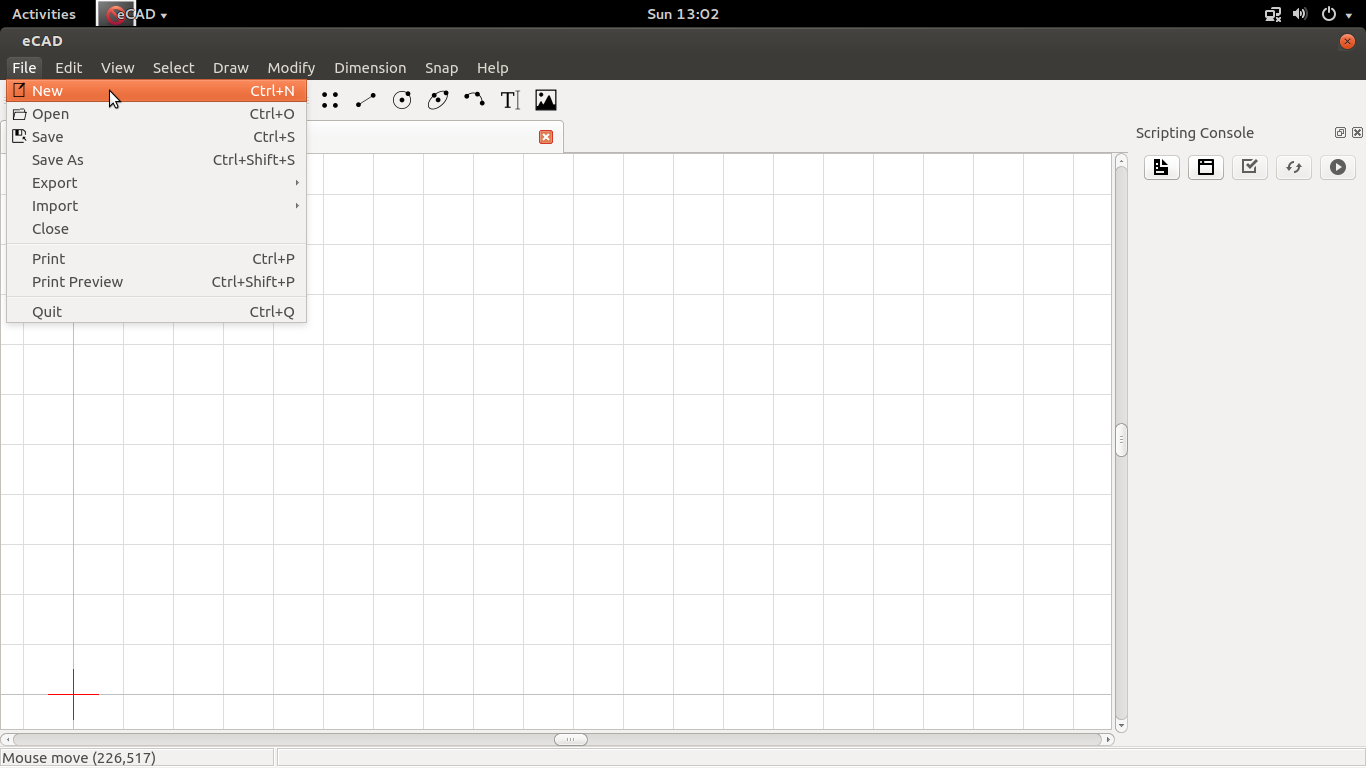
\includegraphics[width=0.7\textwidth]{images/filenew.png}
\caption{New Document from file menu}
\end{figure}
\item \textbf{From toolbar}:
Click on the icon for new document. It will be created
\begin{figure}[h!]
\centering
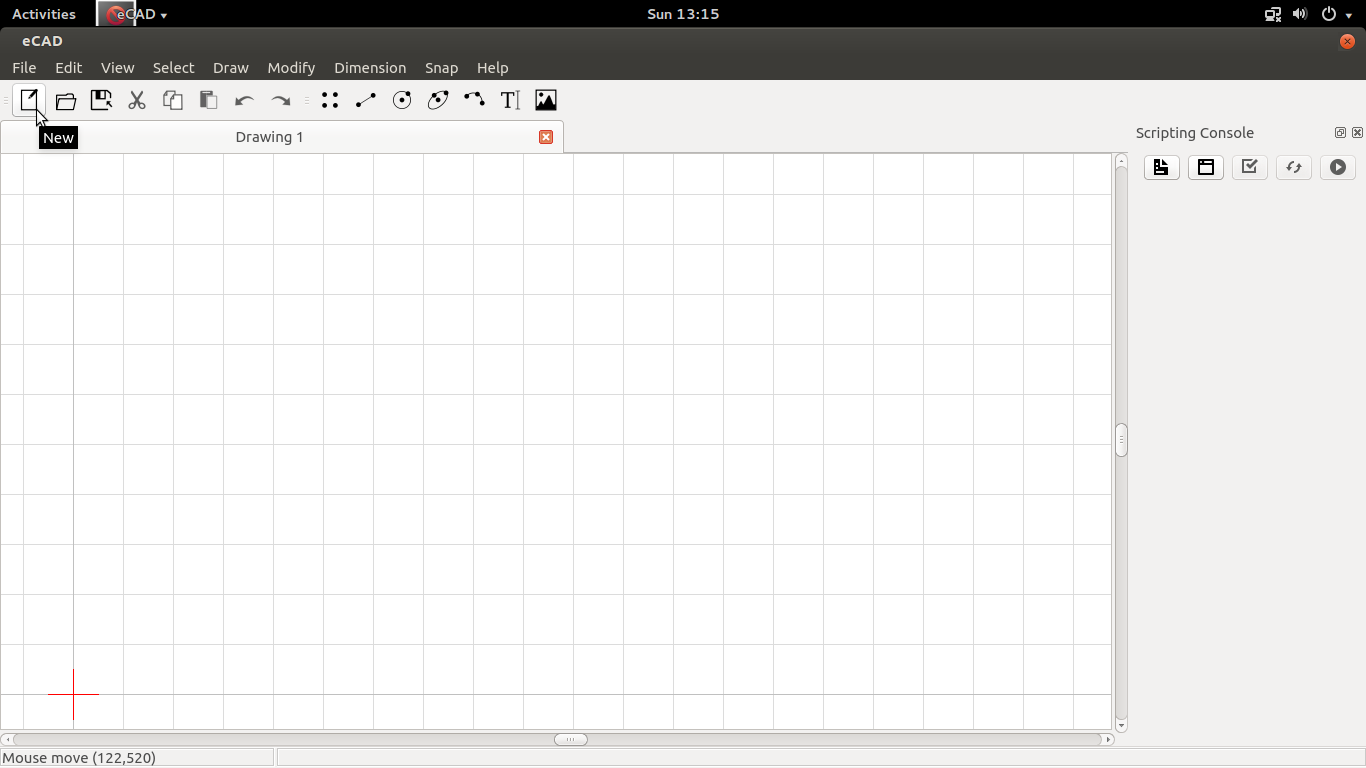
\includegraphics[width=0.7\textwidth]{images/toolnew.png}
\caption{New Document from toolbar}
\end{figure}
\item \textbf{From Shortcut}: Press Ctrl+N a document will be created.
\end{enumerate}
\newpage
\subsection{Saving a Drawing}
We can save the drawing either from file menu or by using shortcut.
\begin{enumerate}
\item \textbf{From File Menu}:
\begin{figure}[h!]
\centering
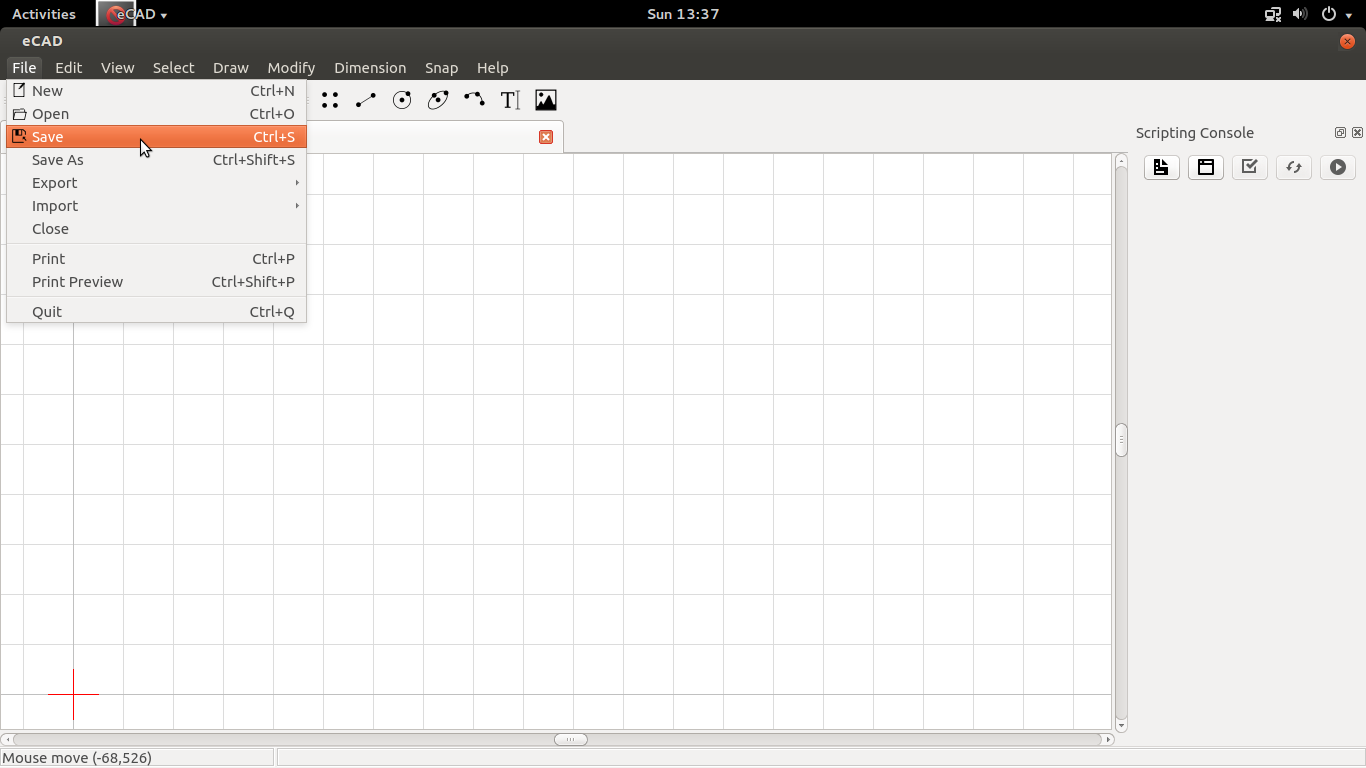
\includegraphics[width=0.7\textwidth]{images/filesave.png}\\
Click File then Save
\end{figure}
\begin{figure}[h!]
\centering
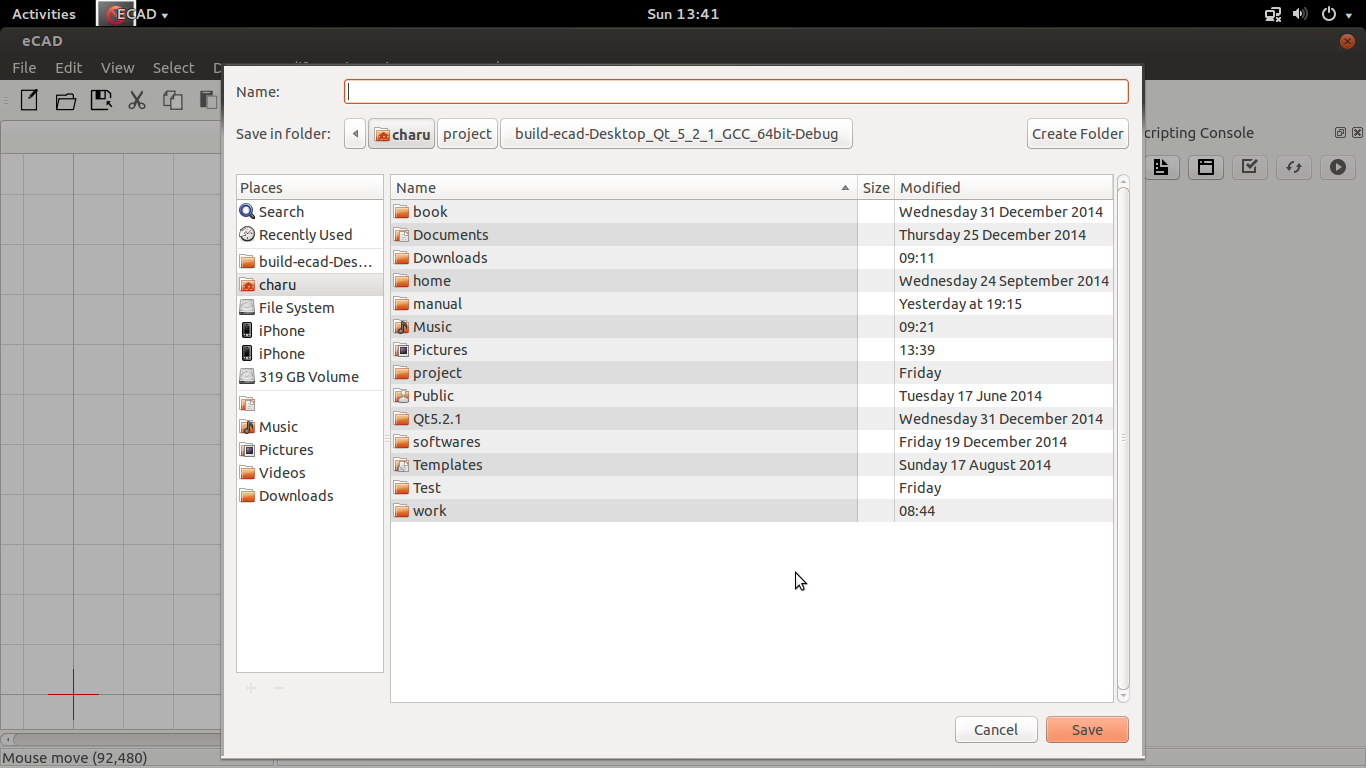
\includegraphics[width=0.7\textwidth]{images/savedialog.png}\\
A dialog box will open then click save.
\end{figure}
\item \textbf{From Toolbar}: Click on the icon in the toolbar to save the file a dialog will open then click save to save he file.
\begin{figure}[h!]
\centering
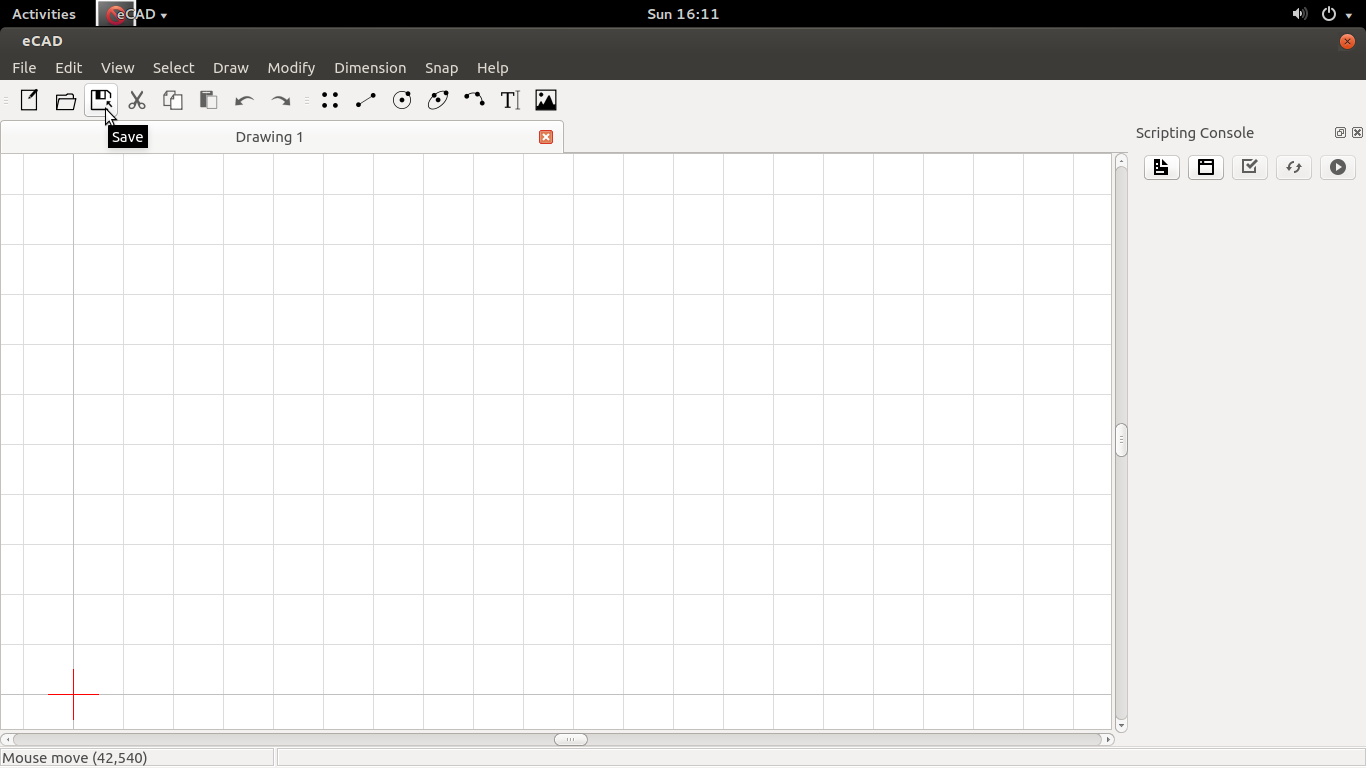
\includegraphics[width=0.7\textwidth]{images/toolsave.png}\\
\end{figure}
\item \textbf{From Shortcut}: Press Ctrl+S to save the file.
\end{enumerate}
\newpage
\subsection{Opening a Document}
We can open the Drawing from menu bar, tool bar or by using shortcut.
 \begin{enumerate}
\item \textbf{From File Menu}:
\begin{figure}[h!]
\centering
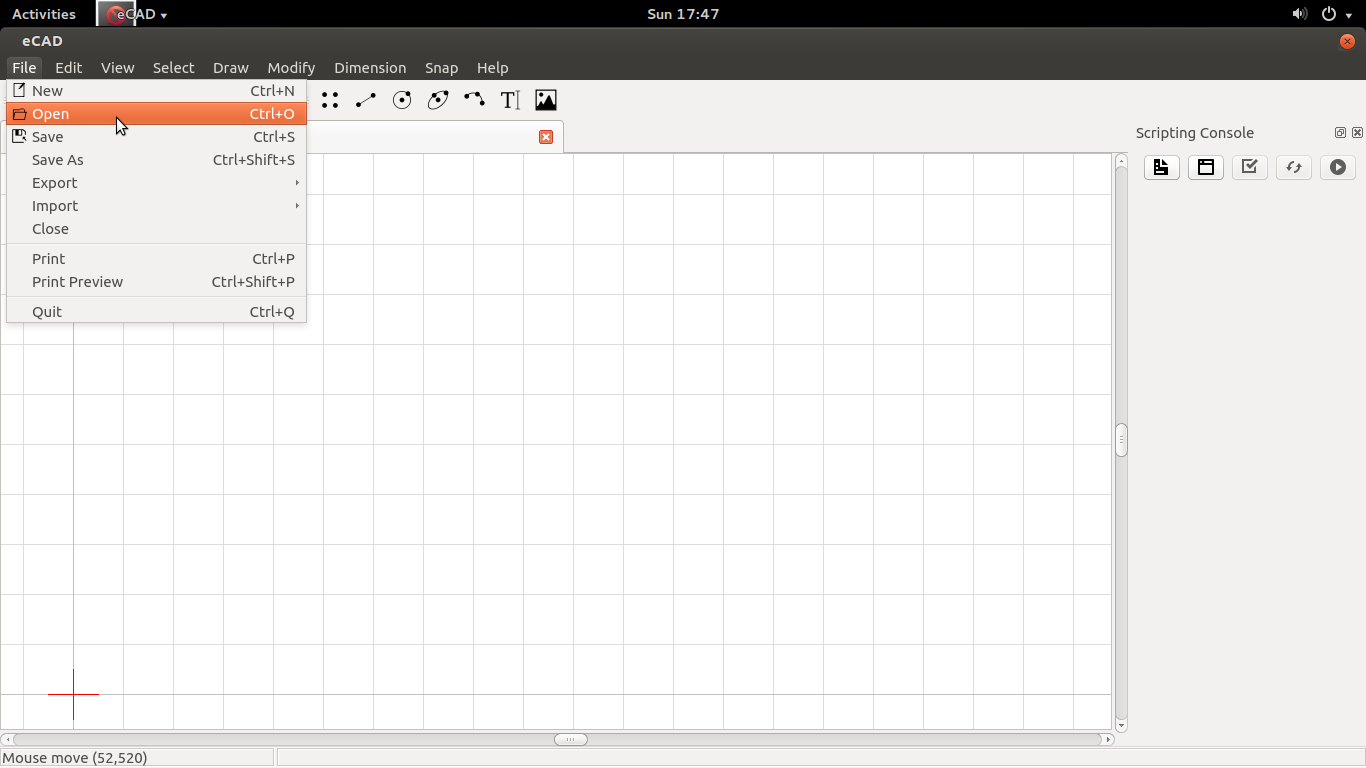
\includegraphics[width=0.7\textwidth]{images/fileopen.png}\\
Click File then Open
\end{figure}
\begin{figure}[h!]
\centering
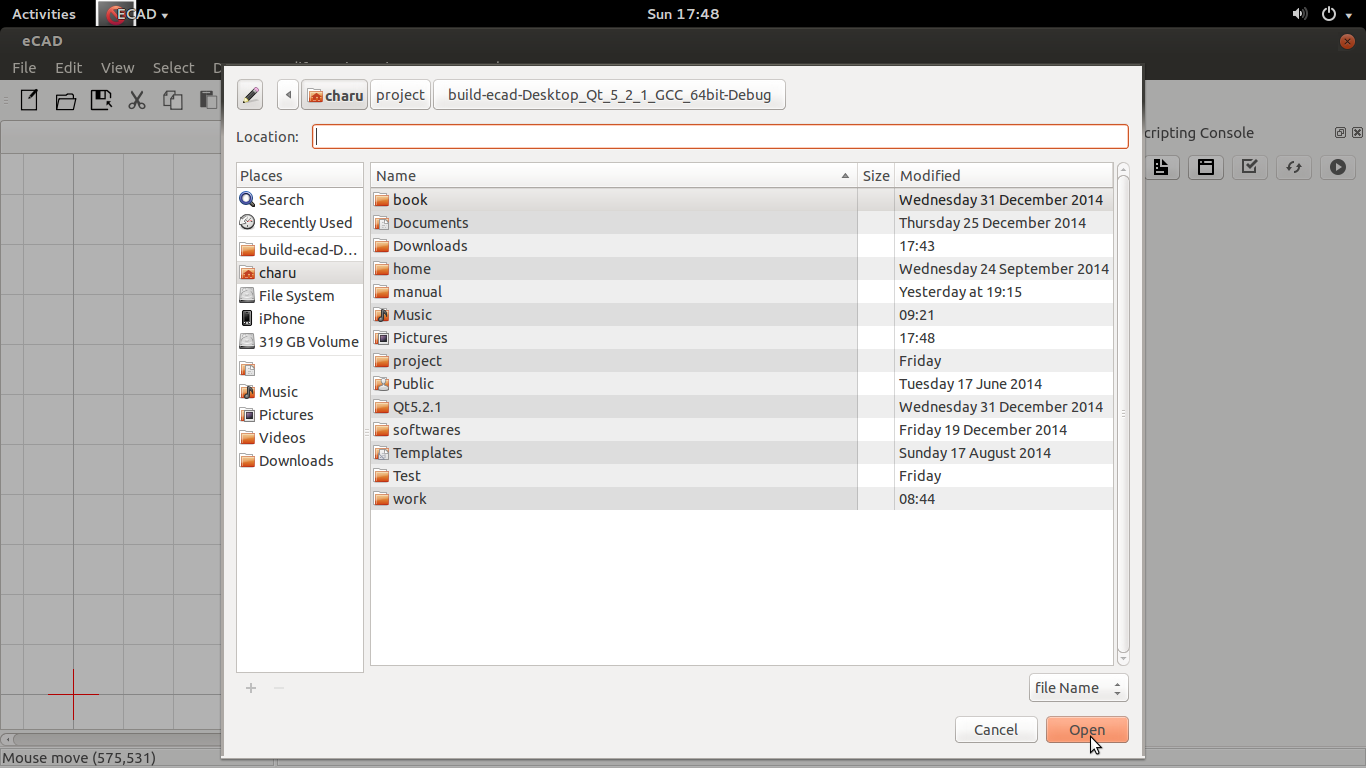
\includegraphics[width=0.7\textwidth]{images/opendialog.png}\\
A dialog box will open then click open.
\end{figure}
\newpage
\item \textbf{From Toolbar}: Click on the icon in the toolbar to open the file a dialog will open then click open to view the file.
\begin{figure}[h!]
\centering
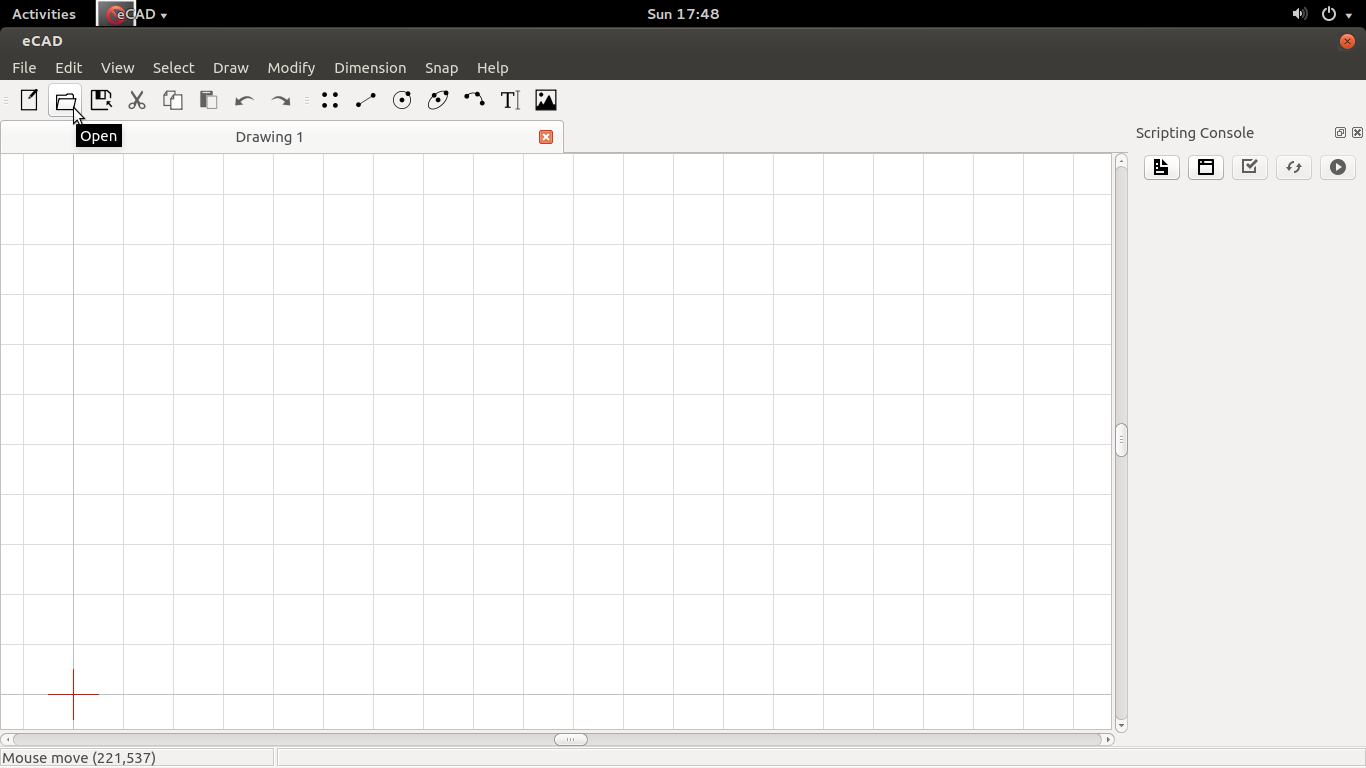
\includegraphics[width=0.7\textwidth]{images/toolopen.png}\\
\end{figure}
\item \textbf{From Shortcut}: Press Ctrl+O to open the file.
\end{enumerate}ar
\newpage
\section{Creating Entities}
There are various ways in eCAD to draw entities. One can draw entities using draw menu, toolbar, shorcuts or commands. Each way is explained in detail as follows:
\subsection{Draw Menu}
We can draw the each entity using draw menu whether its point, line, circle, arc, ellipse, text or image. The way for each entity is described below.
\begin{figure}[h!]
\centering
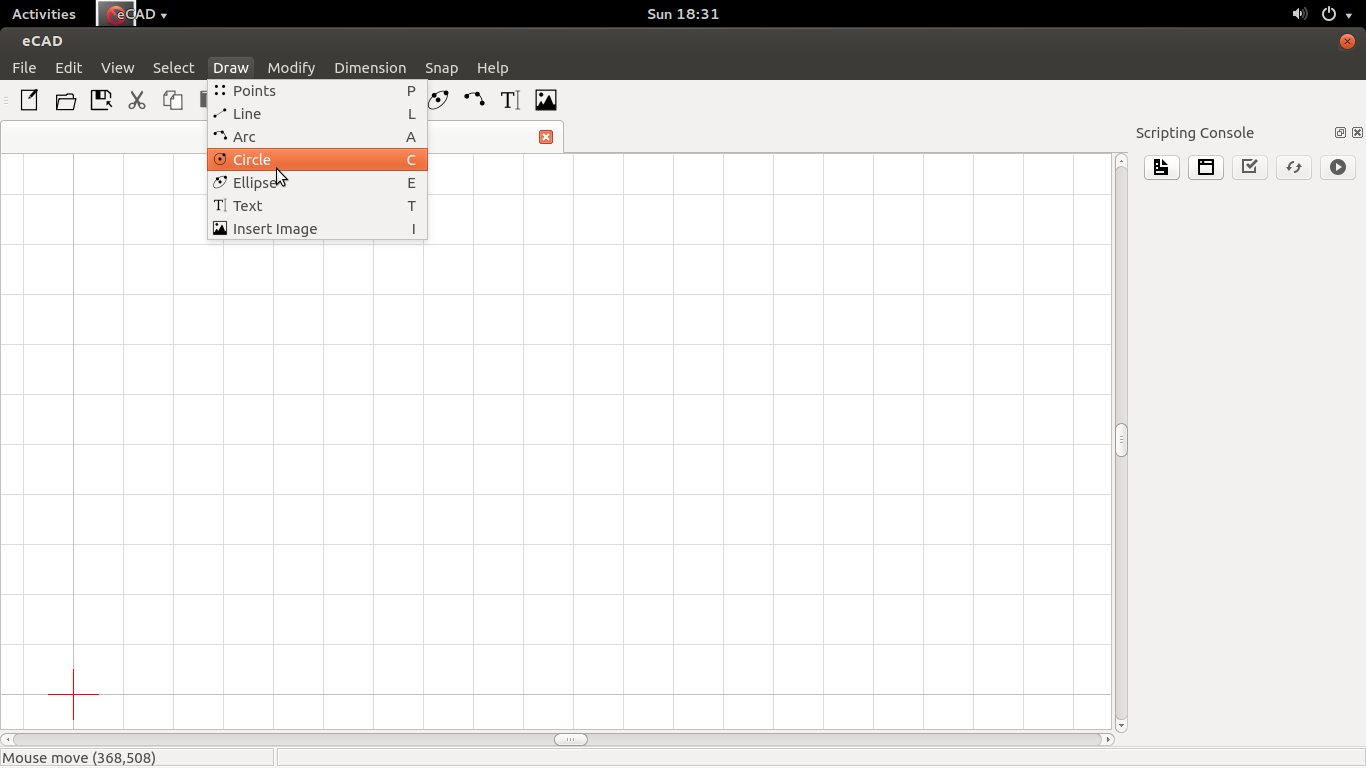
\includegraphics[width=0.7\textwidth]{images/drawmenu.png}\\
\end{figure}
\begin{enumerate}
\item \textbf{Point}
\begin{itemize}
\item Click on point in Draw menu
\item Then click anywhere on working space
\item This will create the point at that location.
\end{itemize}
\item \textbf{Line}
\begin{itemize}
\item Click on line in Draw menu
\item Then click first point on working space.
\item Set the second point of line.
\item This will create the line at two points.
\end{itemize}
\item \textbf{Arc}
\begin{itemize}
\item Click on arc in Draw menu
\item Click the start point of the arc
\item Then second click will create any point on the arc
\item Third click will create the end point of the arc
\item This will create our arc
\end{itemize}
\item \textbf{Circle}
\begin{itemize}
\item Click on circle in Draw menu
\item Then click on working area, this will create center point of arc
\item Second click will create any point on the circle and using first and second click radius of circle is calculated
\item This will create a circle.
\end{itemize}
\item \textbf{Ellipse}
\begin{itemize}
\item Click on point in Ellipse menu
\item Then click on graphics view this will create a center point of ellipse
\item After second click minor radius is calculated
\item After third click major radius is calculated
\item Finally ellipse is calculated
\end{itemize}
\item \textbf{Text}
\begin{itemize}
\item Click on text in Draw menu
\item Then click anywhere on working space
\item This will create a text box in which we can enter the text
\end{itemize}
\item \textbf{Image}
\begin{itemize}
\item Click on image in Draw menu
\item A dialog box will open, select an image to be inserted in it.
\item Then set the image where you want to set.
\end{itemize}
\end{enumerate}

\subsection{Toolbar}
Also we can draw the entities using the toolbar. The entities are in standard toolbar.
\begin{figure}[h!]
\centering

\includegraphics[width=0.7\textwidth]{images/entitytoolbar.png}\\
\end{figure}
\begin{enumerate}
\item \textbf{Point}
\begin{figure}[h!]
\centering

\includegraphics[width=0.05\textwidth]{images/point.jpg}\\
\end{figure}
\begin{itemize}
\item Click on above icon in toolbar
\item Then click anywhere on working space
\item This will create the point at that location.
\end{itemize}
\item \textbf{Line}
\begin{itemize}
\begin{figure}[h!]
\centering

\includegraphics[width=0.05\textwidth]{images/line.jpg}\\
\end{figure}
\item Click on above icon in toolbar
\item Then click first point on working space.
\item Set the second point of line.
\item This will create the line at two points.
\end{itemize}
\item \textbf{Arc}
\begin{figure}[h!]
\centering

\includegraphics[width=0.05\textwidth]{images/arc.jpg}\\
\end{figure}
\begin{itemize}
\item Click on above icon in toolbar
\item Click the start point of the arc
\item Then second click will create any point on the arc
\item Third click will create the end point of the arc
\item This will create our arc
\end{itemize}
\item \textbf{Circle}
\begin{figure}[h!]
\centering

\includegraphics[width=0.05\textwidth]{images/circle.jpg}\\
\end{figure}
\begin{itemize}
\item Click on above icon in toolbar
\item Then click on working area, this will create center point of arc
\item Second click will create any point on the circle and using first and second click radius of circle is calculated
\item This will create a circle.
\end{itemize}
\item \textbf{Ellipse}
\begin{figure}[h!]
\centering

\includegraphics[width=0.05\textwidth]{images/ellipse.jpg}\\
\end{figure}
\begin{itemize}
\item Click on above icon in toolbar
\item Then click on graphics view this will create a center point of ellipse
\item After second click minor radius is calculated
\item After third click major radius is calculated
\item Finally ellipse is calculated
\end{itemize}
\newpage
\item \textbf{Text}
\begin{figure}[h!]
\centering

\includegraphics[width=0.05\textwidth]{images/text.jpg}\\
\end{figure}
\begin{itemize}
\item Click on above icon in toolbar
\item Then click anywhere on working space
\item This will create a text box in which we can enter the text
\end{itemize}
\item \textbf{Image}
\begin{figure}[h!]
\centering

\includegraphics[width=0.05\textwidth]{images/image.jpg}\\
\end{figure}
\begin{itemize}
\item Click on above icon in toolbar
\item A dialog box will open, select an image to be inserted in it.
\item Then set the image where you want to set.
\end{itemize}
\end{enumerate}

\subsection{Shortcuts}
We can even create the entities using the shorcut keys.
\begin{enumerate}
\item \textbf{Point}
\begin{itemize}
\item Press P.
\item Then click anywhere on working space
\item This will create the point at that location.
\end{itemize}
\item \textbf{Line}
\begin{itemize}
\item Press L
\item Then click first point on working space.
\item Set the second point of line.
\item This will create the line at two points.
\end{itemize}
\item \textbf{Arc}
\begin{itemize}
\item Press A
\item Click the start point of the arc
\item Then second click will create any point on the arc
\item Third click will create the end point of the arc
\item This will create our arc
\end{itemize}
\item \textbf{Circle}
\begin{itemize}
\item Press C
\item Then click on working area, this will create center point of arc
\item Second click will create any point on the circle and using first and second click radius of circle is calculated
\item This will create a circle.
\end{itemize}
\item \textbf{Ellipse}
\begin{itemize}
\item Press E
\item Then click on graphics view this will create a center point of ellipse
\item After second click minor radius is calculated
\item After third click major radius is calculated
\item Finally ellipse is calculated
\end{itemize}
\item \textbf{Text}
\begin{itemize}
\item Press T
\item Then click anywhere on working space
\item This will create a text box in which we can enter the text
\end{itemize}
\item \textbf{Image}
\begin{itemize}
\item Press I
\item A dialog box will open, select an image to be inserted in it.
\item Then set the image where you want to set.
\end{itemize}
\end{enumerate}
\newpage
\section{Selecting Entities}
eCAD also provides the option to select the entities. User may select the entities either through the mouse clicks or through the Select Menu.
\subsection{Using Mouse}
eCAD allows the user to select one or multiple entities.
\begin{enumerate}
\item \textbf{Selecting single entity:} User may select single entity by simply clicking on that entity.
\begin{figure}[h!]
\centering
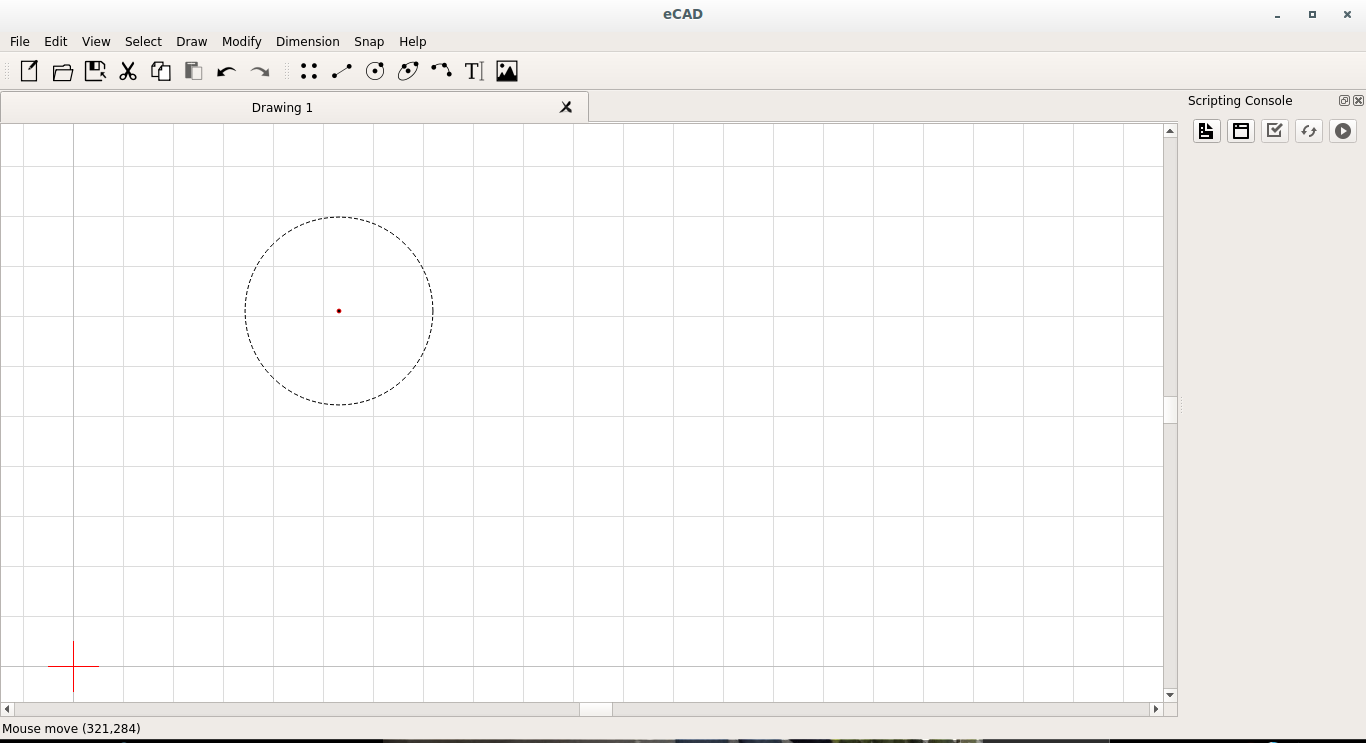
\includegraphics[width=0.5\textwidth]{images/mouseSelect.png}
\end{figure}
\item \textbf{Selecting multiple entities:} Dragging the mouse over the entities will allow one to select them.
\begin{figure}[h!]
\centering
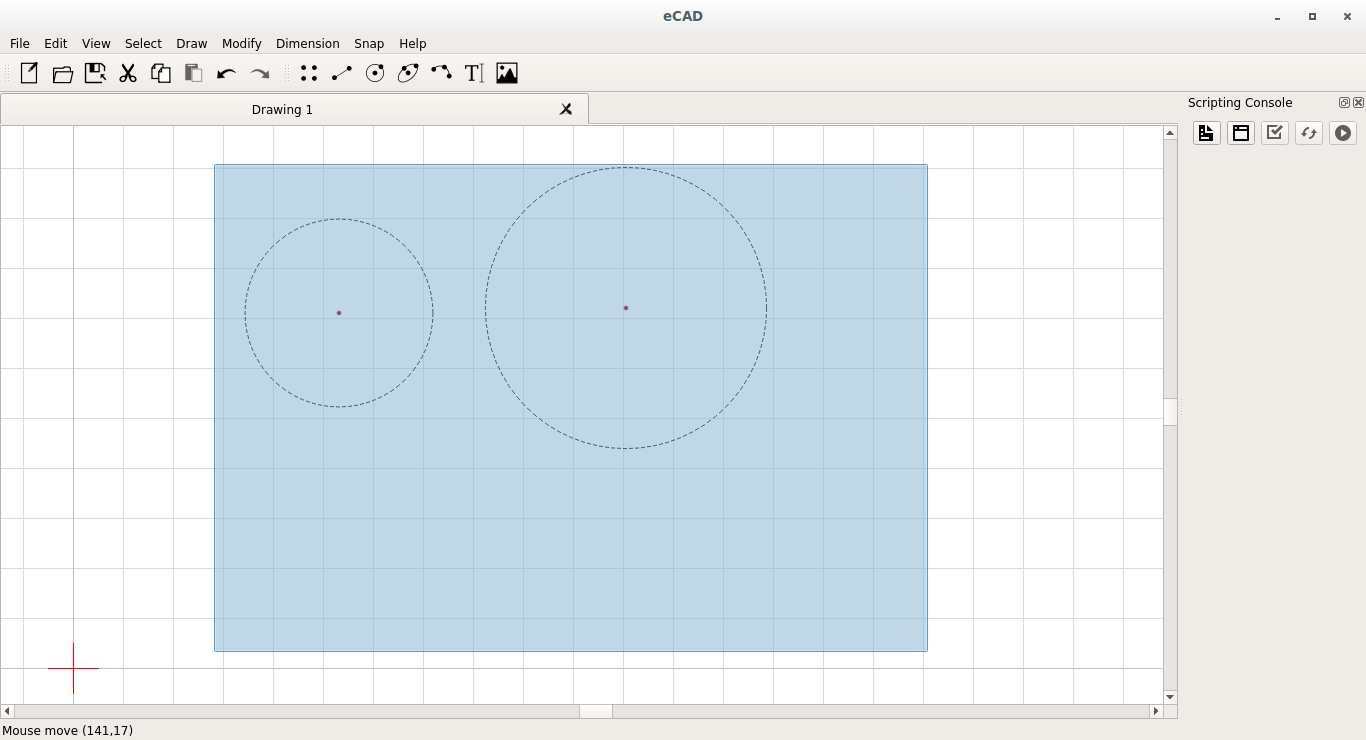
\includegraphics[width=0.5\textwidth]{images/multiple.png}
\end{figure}
\end{enumerate}
\subsection{Select Menu}
Select Menu provides various options to select the entities. Select menu options are explained below:
\begin{enumerate}
\item \textbf{Select All:} This option allows to select all the entities that are currently present on the workspace.
\item \textbf{DeSelect All:} This option allows to deselect all the entities that were currently selected.
\item \textbf{Select Entity:} This option is valid for the single entity that provides user to select the entity, if there is only one entity currently visible.
\item \textbf{Select Window:} Clicking this option would give a user a message to drag the mousein the drawing area to make selection using window and you may drag the mousein to make selection.
\begin{figure}[h!]
\centering
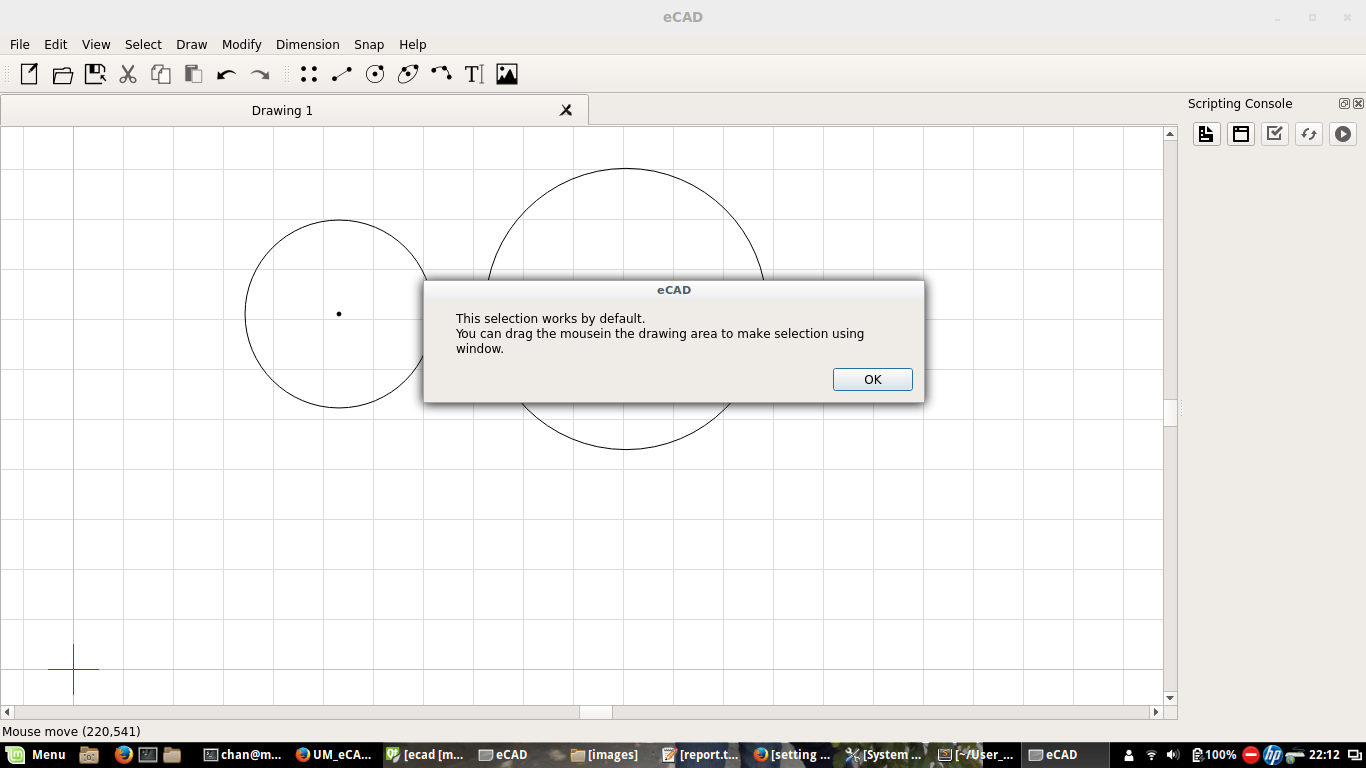
\includegraphics[width=0.9\textwidth]{images/messsage.png}
\end{figure}
\item \textbf{DeSelect Window:} This would allow the user to deselect the entities, selected using Select Window.
\item \textbf{Invert Selection:} Invering selection will make selected entities deselected and vice versa.
\end{enumerate}
\newpage
\section{Operations}
There are various operations that are performed in eCAD.
\subsection{Move}
One can move the entity from one location to other according to user requirement. One can also move multiple entities from one location to another. 
\subsection{Cut, Copy and Paste}
Cut, Copy and paste are one of the important features which need to be embended in any CAD software. Without this any software is incomplete. We can either perform above actions from context menu or from file menu.
\begin{enumerate}
\item \textbf{From Context Menu}
\begin{itemize}
\item Cut: To cut select the entity and right click on that entity then select cut. 
\item Copy: To copy select the entity and right click on that entity then select copy.
\item Paste: To paste the entity right click wherever you want to paste the entity and select paste. 
\end{itemize}
\item \textbf{From Edit Menu}
\begin{itemize}
\item Cut: To cut select the entity and  then select cut. 
\item Copy: To copy select the entity and  then select copy.
\item Paste: To paste the entity select the position on screen then select paste.
\end{itemize}
\end{enumerate}
\subsection{Delete}
We can delete the entity either by using keyboard keys or from Menu.
\begin{enumerate}
\item \textbf{From keyboard keys}:
Select an entity then press Delete key.
\item \textbf{From Menu}:
Select the entity then press delete from delete menu.
\end{enumerate}
\subsection{Undo/Redo}
We can undo redo either by using shortcuts or from the edit menu.
\begin{enumerate}
\item \textbf{From edit menu}
\begin{itemize}
\item Undo: Click on undo to undo the previous action
\item Redo: Click on redo to redo the action.
\end{itemize}
\item \textbf{From Shorcuts}
\begin{itemize}
\item Undo: Press Ctrl+ Z to undo the previous action
\item Redo: Press Ctrl+Shift+Z to redo the action.
\end{itemize}
\end{enumerate}
\newpage
\section{Actions in eCAD}
\subsection{Panning and Zooming}
Pan and zoom are very useful tools in eCAD. The zoom tool is invaluable when you need to move up close to an entity to work on it. This is especially true when the area is very small, or several lines drawn close together. As you will see in a moment, there are several ways to use zoom. Pan allows you to move the drawing up, down, right, or left. This is especially useful if your drawing is large. Pan and zoom are accomplished by two methods. Either from the menu or using cursor.
\begin{enumerate}
\item \textbf{From Menu}
\begin{itemize}
\item Zoom In: Go to View then click Zoom In to zoom.
\item Zoom Out: Go to View then Click Zoom Out to zoom.
\item Panning: Go to view then click Panning, hand cursor will appear now you can move the screen as you want to do that.
\end{itemize}
\item \textbf{Using cursor}:
Zooming can be achieved by mouse wheel scrolling. By default, wheel scrolling triggers zooming-in/out respectively.
\end{enumerate}

\subsection{Toggling Visibility}
There are various which we can set according to our requirement. Like grid, scripting console, command console, status bar, tool bar etc. It all depends upon user need how user want to see the screen. 
\begin{enumerate}
\item \textbf{Grid}:
\begin{figure}[h!]
\centering
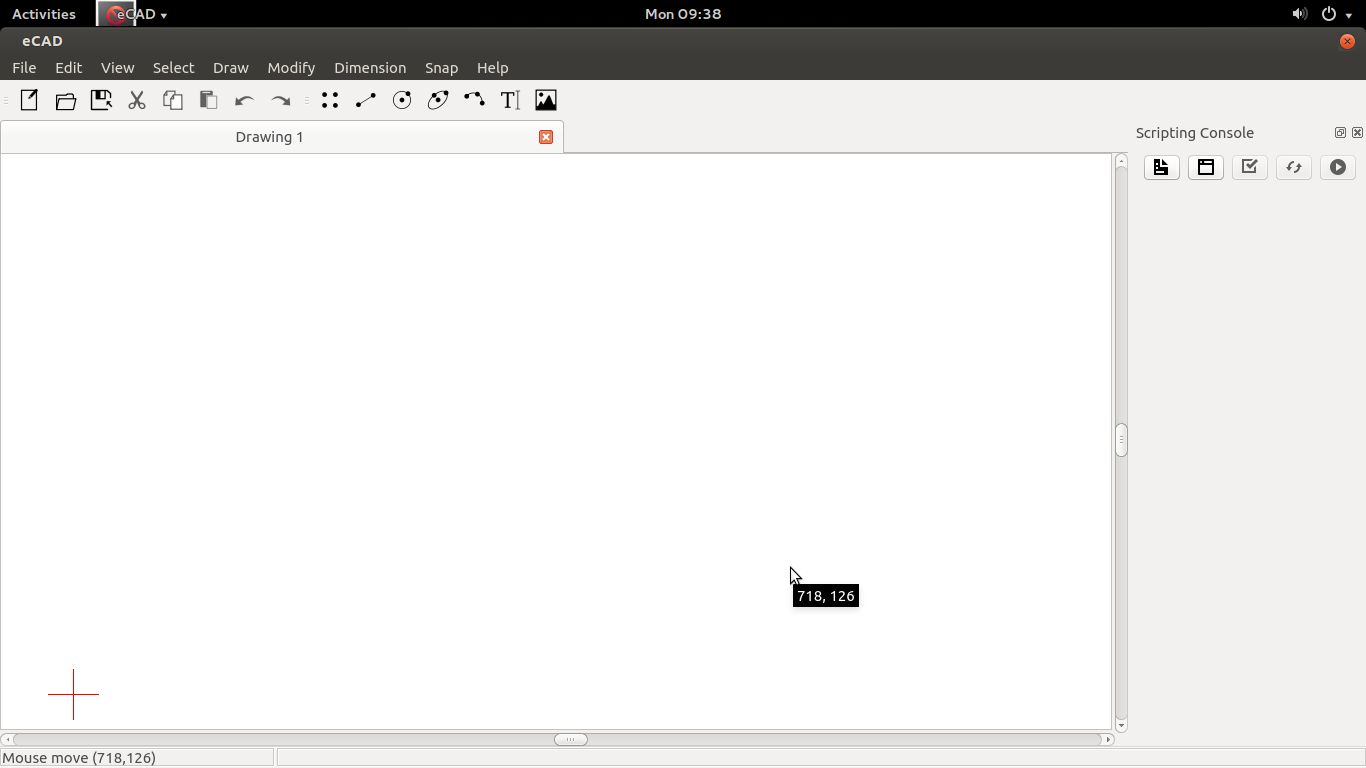
\includegraphics[width=0.7\textwidth]{images/togglegrig.png}\\
Go to View the uncheck the grid Grid will not be visible.
\end{figure}
\newpage
\item \textbf{Scripting Console}:
\begin{figure}[h!]
\centering
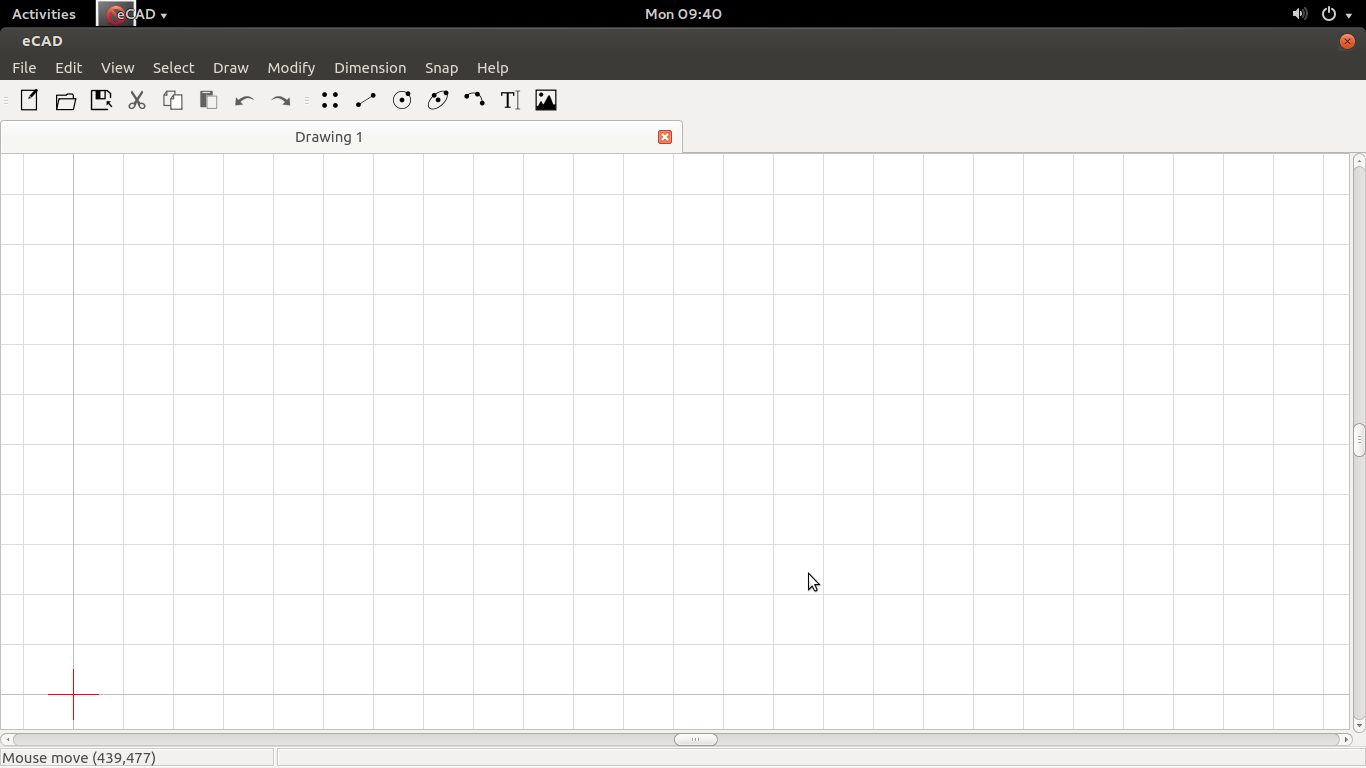
\includegraphics[width=0.7\textwidth]{images/togglescripting.png}\\
Go to View then Toolbars and uncheck the scripting. Scripting widget will get closed.
\end{figure}
\item \textbf{Command Console}:
\begin{figure}[h!]
\centering
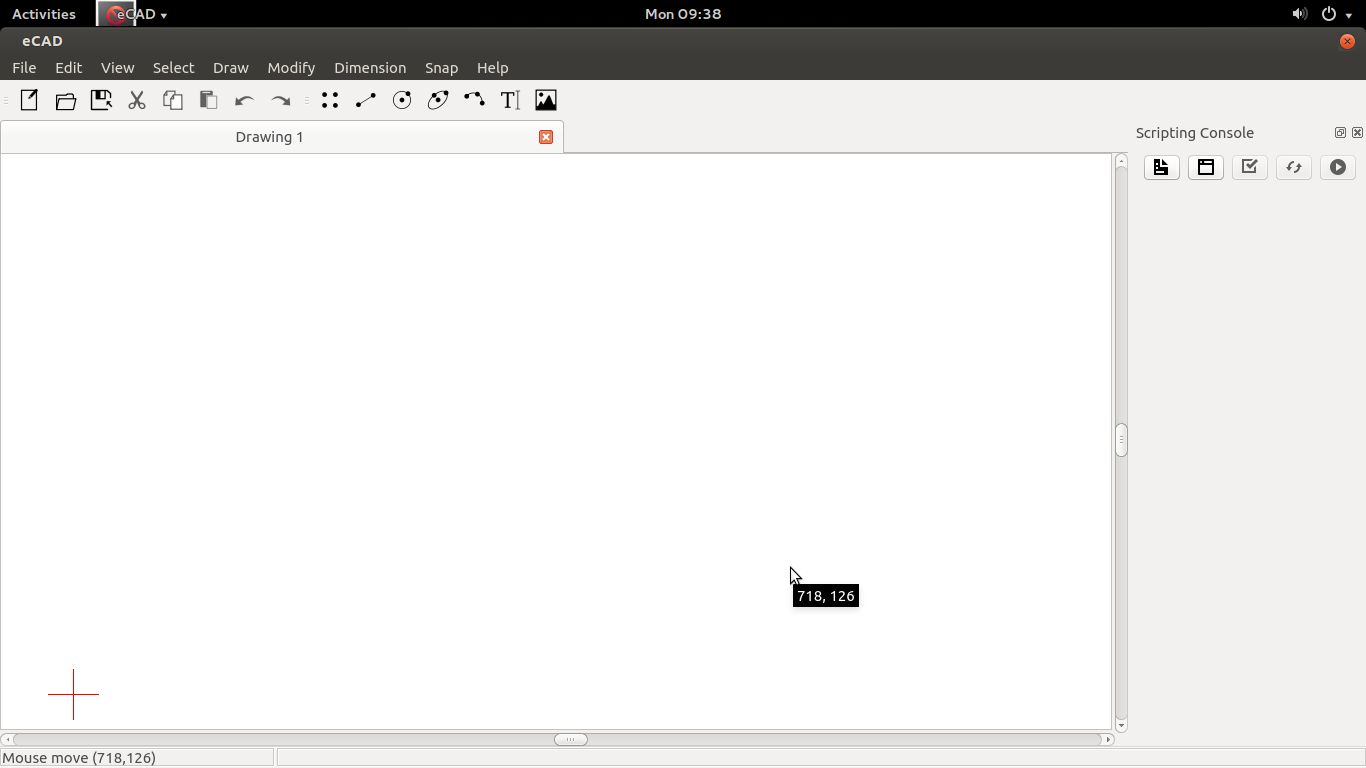
\includegraphics[width=0.7\textwidth]{images/togglegrig.png}\\
Go to View then Toolbars and check the command console it will be visible. By default command console is unchecked
\end{figure}
\newpage
\item \textbf{Status Bar}:
\begin{figure}[h!]
\centering
\includegraphics[width=0.7\textwidth]{images/togglestatus.png}\\
Go to View and uncheck the status bar the status bar will not be visible
\end{figure}
\item \textbf{Tool Bar}:
\begin{figure}[h!]
\centering
\includegraphics[width=0.7\textwidth]{images/toggletool.png}\\
Go to View then Toolbars and uncheck the toolbar the standard toolbar which contains all the entities will not be visible.
\end{figure}
\end{enumerate}
\newpage
\section{Scripting}
A script is a macro, a list of commands that you can run all at once, and as many times as necessary, allowing you to automate tasks that would take a long time if you did them manually. Scripts can be very powerful and you can run them on  objects in one drawing, or on many drawings. Scripts have been around for many years and many people have a library of many scripts that they use.\\
\begin{itemize}
\item First step for scripting is to create a script file. Click on new icon in scripting console
\item A dialog box will open save that file with .js extention
\item Start writing the script 
\item After writing the script click on execute icon. This will create a drawing in the drawing  area. 
\end{itemize}
There are various commands for each entity. Different commands for different entities. They are almost similar difference is in the parameters which we have to pass for scripting. Let's discuss each command in detail.
\subsection{Point}
To create a point type cad.point(x coordinate, y coordinate).\\
For example cad.point(500,300). Then execute it a point will be made.
\subsection{Line}
To create a line cad.line(start x coordinate, start y coordinate, end x coordinate, end y coordinate).\\
For example cad.line(150,100,200,210);
\subsection{Circle}
To create an arc cad.circle(center x coordinate, center y coordinate, radius).\\
For example cad.circle(50,50,30);
\subsection{Ellipse}
To create an ellipse cad.ellipse(center x coordinate, center y coordinate, major radius, minor radius).\\
For example cad.ellipse(50,50,60,30);
\subsection{Arc}
To create an arc cad.arc(start x coordinate, start y coordinate, end x coordinate, end y coordinate).\\
For example cad.arc(120,130,233,321,456,546);
\subsection{Text}
To create text cad.text(start x coordinate, start y coordinate, text)\\
For example cad.text(420,520,”hello”);
\end{document}
